\section{Evaluation}

\if 0
\begin{changes}
We evaluate how reliably we can detect and parse explainable regions in online programming help, and conduct an in-lab usability study to observe how programmers use \glspl{exp} when modifying unexplained code.
\end{changes}
First, how reliably can automatic explanations could be generated for the expanse of different formats of online tutorials?
Second, can \glspl{exp} help programmers modify existing, unexplained code without having to consult additional documentation?
We answered the first question through collecting a corpus of online tutorials and measuring the detection accuracy of our \Glspl{name} for the languages we support.
We address the second question through an in-lab study with programmers modifying unexplained code to perform new tasks, aided by \Glspl{name}.
\fi
%
\subsection{Detection and Parsing Accuracy}
\begin{changes}
While users can explicitly select text that they want to have explained with the \Glspl{name} addon, automatic preprocessing and detection of explainable regions can provide improved information scent.
In this section, we assess our \Glspl{name}' accuracy in detecting explainable regions.

We collected a set of online programming help pages that used the languages of each of our \Glspl{name}.
To assemble this corpus, we formulated queries for tutorials.
Using the API for StackOverflow, a popular programming Q\&A site, we extracted the most frequent triplets of tags that included each language's tag.
% These triplets of tags related to tasks (`mod-rewrite redirect regex') as well as  languages and libraries (`casperjs css-selectors javascript').
For these triplets, we queried Google with the triplet and the word `tutorial' (e.g. `mod-rewrite redirect regex tutorial'), yielding around 200 programming help documents per language. % that covered a variety of different programming tasks.
After choosing random sample of 50 documents for each language from this set, 
we manually extracted the element and character location of all uses of each language, yielding more than 100 examples per language.
We ran the \Glspl{name} on each document and compared the regions the \Glspl{name} found to those we extracted by hand.

With the current \Glspl{name}, we observe 95\% precision (129/136) and 64\% recall (129/203) for wget, 62\% precision (164/238) and 48\% recall (164/343) for CSS selectors, and 78\% precision (100/129) and 14\% recall (100/445) for regular expressions.
Our detectors achieve high precision yet low recall.
Major reasons for low recall are:
\emph{(a)} wget: we fail to reliably detect code examples within sentences of text.
\emph{(b)} selectors: we scan only `pre' and `code' nodes while skipping `div' nodes.
\emph{(c)} regular expressions: while we write rules to reliably detect regular expressions in some contexts (Apache server configs, sed, grep, and Javascript), rules are missing for others (Python, Perl, etc.).
We can compensate for low recall by extending the browser addon to allow programmers to request explanations for arbitrary text.
Recall may be further improved by incorporating a machine learning approach to recognizing commands (e.g.,~\cite{pavel_browsing_2013}).

\if 0
\begin{table}
\caption{Accuracy of our explainable region detection.}
\label{tab:detection_accuracy}
\centering
\begin{tabular}{llc}
\toprule
\headrow{Language} & \headrow{Precision} & \headrow{Recall} \\
\midrule
wget & 84\% & 61\% \\ \midrule
CSS selectors & 69\% & 48\% \\ \midrule
RegEx & 78\% & 14\% \\ \bottomrule
\end{tabular}
\end{table}
\fi

As we built our CSS selector parser by hand, we discuss its accuracy parsing the ground truth selectors we extracted during the detection tests.
% We ran our parser against the CSS selectors we extracted from the previous tests as part of our ground truth to see how often it could parse the selectors from the past step without error. \marti{Don't know what you are talking about here.}
Of the 334 selectors that we labeled, 322 (96.4\%) parsed without error.
Of the 12 that failed to parse, 10 of them could not be lexed as they included incorrectly-formatted characters in the original HTML markup or jQuery-specific pseudo-classes that do not belong to the CSS syntax.
By leaving out these invalid selectors, our parser was able to successfully parse 332 / 334 selectors found online (99.4\%).

\end{changes}

\subsection{In-Lab Usability Study}

We conducted a usability study to understand how \Glspl{name}-generated \glspl{exp} affected programmers' ability to perform code modification tasks with online example code.
We recruited 9 programmers from university listservs for undergraduate and graduate students in computer science and information science.
All participants had at least two years of programming experience, with a median of 4 years of experience in their longest-used language.

Each participant attempted 8 code modification tasks (plus 2 practice tasks) using two different languages: CSS selectors and wget.
For each language the 4 coding tasks increased in difficulty with the fourth being especially tricky.

\begin{changes}
Each code modification asked a participant to:
\begin{enumerate}
    \item Read a task.  For example: ``modify the [wget] command so it does not automatically fetch the images necessary to display the webpage.''
\item View a snippet that is unrelated to the specific modification task, but that contains some clue on how to do it.  For example, a StackOverflow post that includes, but doesn't explain, this command:
\vspace{.2em}
\snippet{wget --random-wait -r -p -nd -e robots=off -A".pdf"  -U mozilla http://math.stanford.edu/undergrad/}
\vspace{.6em}
\item Write and test code against a condition we provide.
\end{enumerate}

After reading the snippet, participants could use any resources they wanted to, including web search, to complete the task.
To make the code examples similar to what a programmer would find when searching for help, we adapted snippets from StackOverflow questions or answers.
Tasks asked participants to modify code, as we hoped to find whether the \Glspl{name} provided enough understanding of the code to help programmers perform a practical task.
\end{changes}

\if 0
Example tasks included:
\begin{itemize}

\item
Snippet (excerpt):

\item
Snippet (excerpt):

\snippet{wget -r -np -N [url] \\}

Task: modify the command to overwrite all files downloaded, even if they have not been updated remotely.

\item

Snippet (excerpt, 1 of 15 lines):

\snippet{\$(`input[id\textasciicircum=``ProductId\_'']')\textbackslash \\  .each(function () \{ }

Task: write a selector that selects only the button elements with IDs starting with bid

\end{itemize}
\fi
%
\begin{changes}
In one condition, snippets were enhanced with \glspl{exp}.
The explanation did not contain exactly the missing information to complete the task.
For example, for wget tasks, participants were shown descriptions of all options and asked to discover and modify or remove only those relevant to the task.
While these tasks limit the generalizability of our study, we believe that it shows that \Glspl{name} can help in the situations we devised and tested.

Participants viewed \glspl{exp} for alternating tasks so we could observe differences in how they approached the tasks with and without them; order of exposure to \glspl{exp} was counter-balanced across participants. 
When in the \gls{exp} condition participants were asked to find and view all \glspl{exp} for the source code after reading the snippet.

Participants were told they would have 5 minutes for each task; if participants had extra time and they had not completed the task, we often asked them to continue so we could observe their problem-solving process.
For this study, the browser addon was not instrumented with visual indicators of explainable regions as this feature was not yet conceived, although \glspl{exp} were pre-fetched.
We asked participants to ``think aloud'' as they performed these tasks.

\end{changes}

\if 0
\begin{figure}
\centering
\framebox{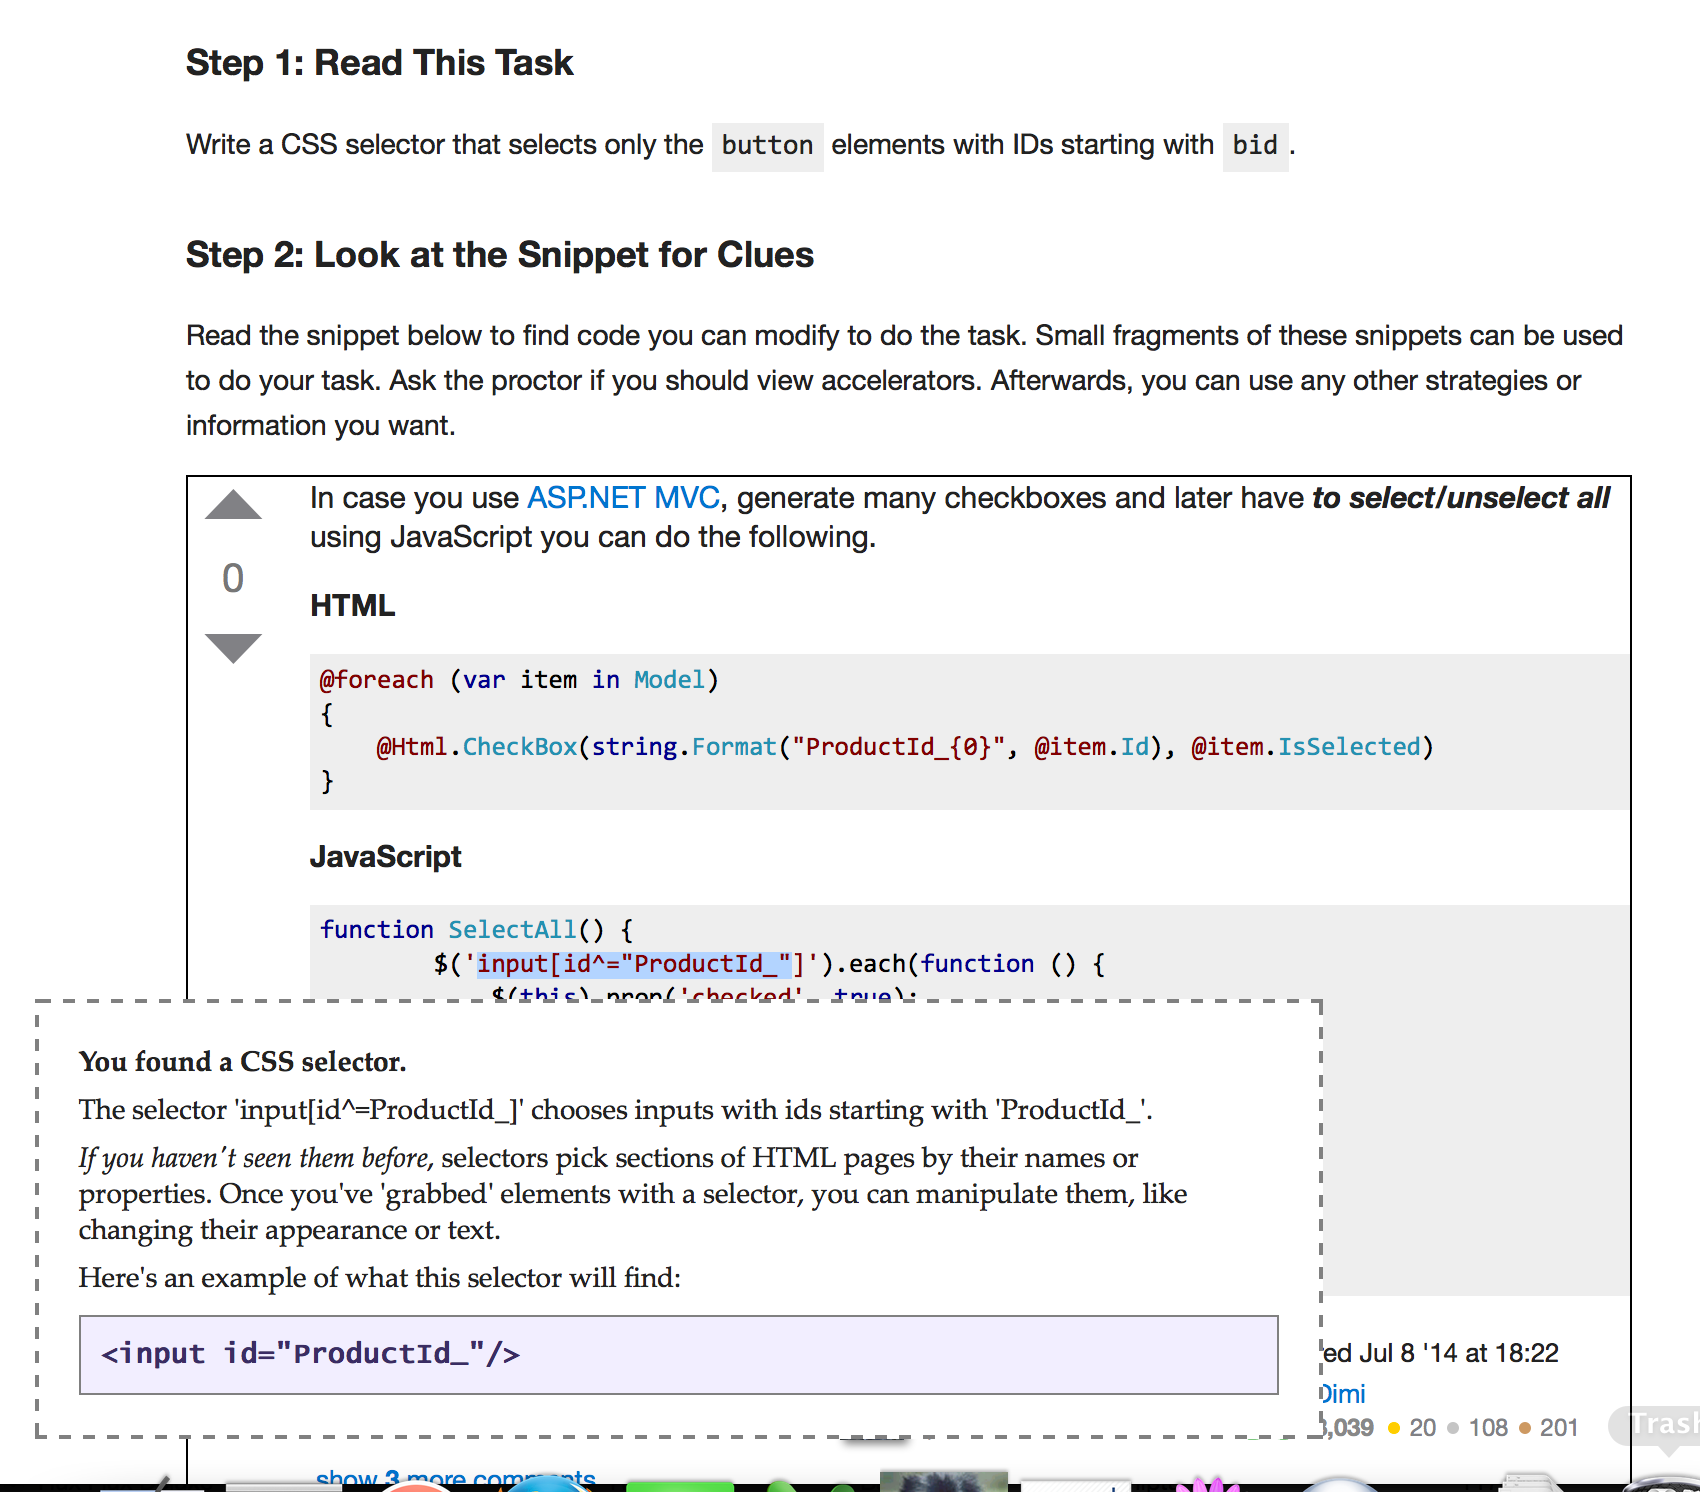
\includegraphics[width=\columnwidth]{figures/study_snippet}}
\caption{An example snippet shown as a clue for a code modification task, accompanied by a \gls{exp} that a participant in our study would have viewed if they were instructed to do so in this task.}
\label{fig:study_snippet}
\end{figure}
\fi
%%This ordering was counterbalanced across participants so that we could see all tasks performed both with and without \Gls{name}-generated \glspl{exp}.

\subsection{Results}

Our primary goal in observing participants was to determine if \Gls{name}-generated \glspl{exp} were helpful  during code modification tasks and reduced the need to reference additional documentation.
In the discussion below, we refer to our participants as $P{1-9}$.

\subsubsection{\Glspl{exp} Help Programmers Modify Code Without Using Other Documentation}

\begin{figure}
\centering{%
\subfigure{%
    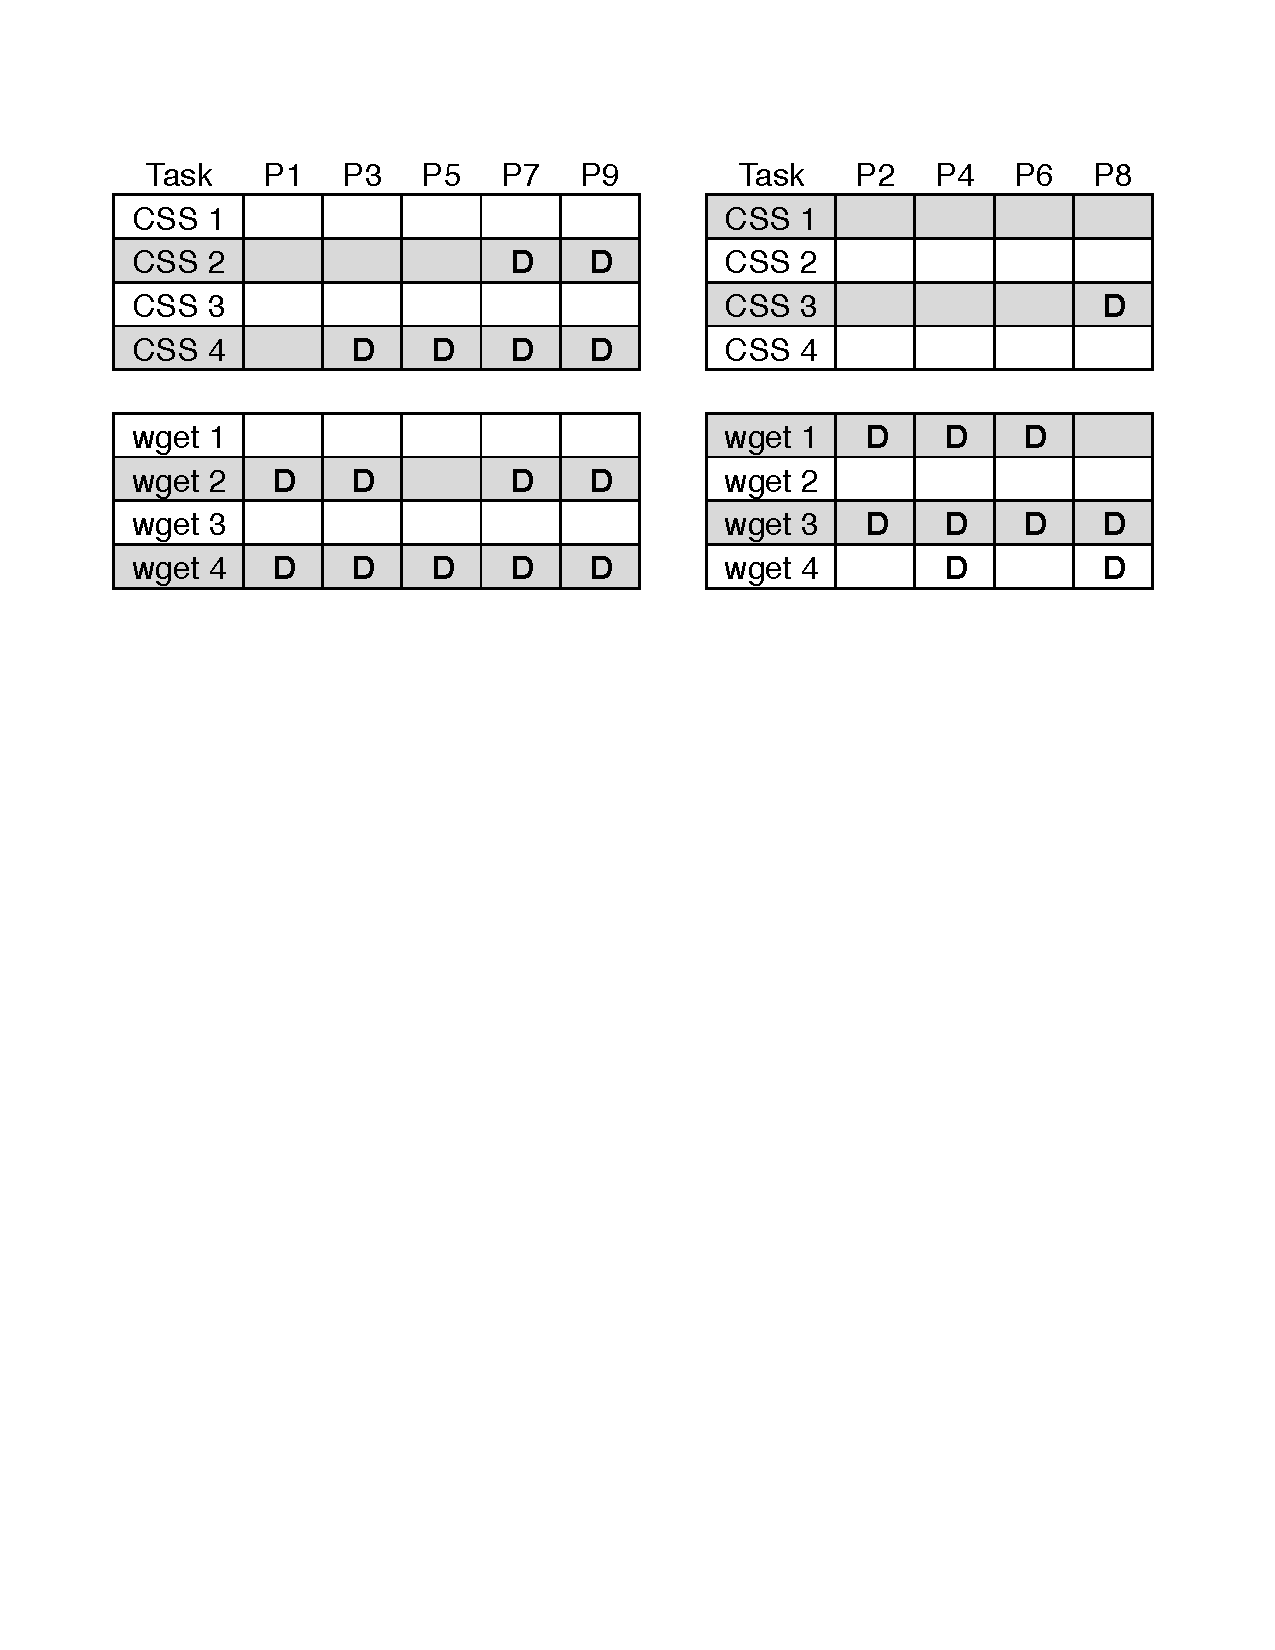
\includegraphics[width=\columnwidth]{figures/doc_accesses}\label{fig:doc_accesses_log}
}
\subfigure{%
    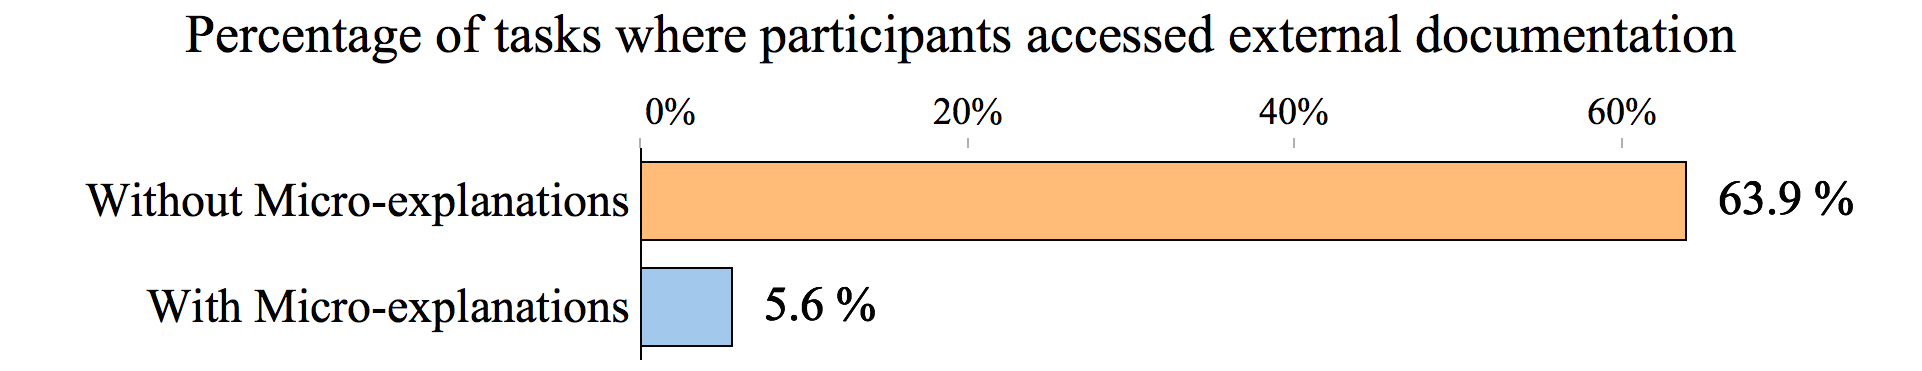
\includegraphics[width=\columnwidth]{figures/doc_accesses_bars}\label{fig:doc_accesses_bars}
}
\caption{%
Tasks for which participants sought additional documentation beyond the snippet. In white rows, participants used \glspl{exp}; in gray rows, they did not.
A cell is marked with the letter `D' if a participant accessed external documentation during that task.
Participants used additional documentation for 63.9\% of tasks when \glspl{exp} were not available, and for 5.6\% of tasks when they were available.
}
}
\label{fig:doc_accesses}
\end{figure}

\begin{changes}
When using the \glspl{exp}, 2 out of 36 tasks, or 6\% required external documentation.
However, for those tasks where \glspl{exp} were not available, 63\% of the time participants did indeed access external resources in order to complete the task.
This difference is significant (Fisher's exact test, $p < 0.0001$)
\end{changes}
The wget tasks especially required external help, with \texttt{man} pages and other resources being accessed in 89\% of cases.  
A log of external document accesses is shown in Figure~\ref{fig:doc_accesses}. 


%%In total, out of 72  tasks, participants sought out additional documentation a total of 25 times (Figure~\ref{fig:doc_accesses}).
%%In all wget tasks and in the fourth CSS selector task, a majority of participants without \Glspl{name} viewed documentation at some point while trying to find a solution to the problem.
%%In the all 4 CSS selector tasks and the first 3 wget tasks, no participants with access to the \glspl{exp} sought additional documentation in order to solve the problem.

%Only in the final wget task did any participants with access to \Glspl{name} seek documentation.


These preliminary results suggest that the \glspl{exp} are effective at reducing the need to switch contexts to find relevant programming help  for completing some programming tasks. 
The \gls{exp} aided the programmers in several ways:

{\bf Reducing need to access external documentation.}
Participants were  able to identify which flags had to be removed from wget commands without consulting external documentation, despite not having used wget before ($P4$).
For others, the \gls{exp} affirmed a guess that the participant already had about how to construct a CSS selector ($P1$).

{\bf Context-relevant pattern matching.}
One participant noted that the \glspl{exp} helped  to map flags for a wget command to the higher-level intent of the task ($P4$). 
For the most complex CSS selector task, two participants noted
that the example HTML shown in the \gls{exp} 
provided a pattern of what fields needed to be changed  from the selector in the snippet to capture the element and ID required by the task prompt ($P2$, $P4$).

{\bf Learning programming concepts.}
For another participant with little previous experience with CSS selectors, a \gls{exp} in  the first task provided him with the knowledge needed to write the selector for the next two tasks, one task for which he was not allowed to view \glspl{exp} ($P5$).

\subsubsection{Programmers Without \Gls{exp} Searched External Documentation}

Some of the difficulties participants faced in the no-\gls{exp} condition  highlight the benefits of in-situ help.
Some participants had difficulty searching for programming help on a web search engine (Google) and using the search results.
One participant could not express the symbols `\texttt{\^{}=}' as a query term when searching for the pattern's meaning for CSS selectors.
Her follow-up queries with English language query terms  yielded search results that were not relevant ($P3$).

Participants also had difficulty navigating conventional forms of programming help.
When looking for the \texttt{-r} flag in the \texttt{man} page for wget, participants found that a page-internal search for the flag yielded so many matches that it was difficult to find the desired definition ($P2$, $P4$).
The description of the \texttt{-N} timestamp flag that was relevant to the code modification task was not adjacent to where the flag was introduced, causing one participant to overlook this information ($P3$).

These results underscore the usefulness of context-relevant explanations located within the tutorial text itself.

\subsubsection{Opportunities for Improvement}
In those cases where the \gls{exp} did not aid programmers, there were a few primary causes.

{\bf No visual affordances.} For this study, we did not place visible cues showing where explanations were available.
Some programmers failed to find \glspl{exp} since they had to be explicitly invoked by selecting text.
\shortchange{One participant ($P2$) had to be reminded that he had to click around the snippet to find \glspl{exp} for unexplained code when he had not found all explainable regions.}
\if 0
Although $P2$ eventually found a \gls{exp} that led him to writing a successful CSS selector for the most difficult CSS task, he had to click around the snippet to find it, and did so only upon being reminded by the experimenter that he had not viewed all the \glspl{exp} in the snippet ($P2$).
\fi
Since this study, the browser addon has been instrumented with visual feedback of all regions automatically detected.

{\bf Selection region ambiguity.}
\begin{changes}
At the time of the study, the algorithm we used to summon an explanation for selected text caused irrelevant explanations to appear when users selected text that was a substring of a detected, explained string.
Several participants experienced this problem ($P1$, $P3$, $P5$).
\if 0
For example, one participant selected the text \texttt{<p>} for which no explanation was generated by the explanation server, because no CSS selector starts with a less-than sign.
However, our selection matching algorithm matched this string to the \texttt{p.mainPageMeters} selector for which an explanation \emph{had} been generated by the server.
As a result, this participant viewed an irrelevant explanation for the code fragment he was viewing ($P5$).
More work is required to determine the right balance of fuzziness for the matching algorithm, with perhaps a drop-down menu of choices for alternative matches.
\fi
With the addition of visual information scent, clickable regions now have exactly one correct explanation to overcome this problem in the default case.
However, the mechanics of ``fuzzy'' selection boundaries should be investigated further for when users manually request explanations of a language that are not automatically detected by \Glspl{name} through a right-click.
\end{changes}

{\bf Incomplete explanations.} The  \gls{exp} text may not include enough detail to help programmers  develop adequate mental models of unfamiliar material. For instance,
even after completing all 4 CSS selector tasks, $P5$ appeared to believe that CSS selectors were HTML elements themselves, rather than labels that could fetch them, perhaps confused by the example HTML produced in each \gls{exp}.
That said, the idea of \gls{exp} can be expanded by adding links to fuller tutorial material.
